La aplicación permite cargar datos, indicar preferencias y consultar los horarios. Se elige al estudiante mediante un selector, sin iniciar sesión. El recorrido es \emph{Datos, Estudiantes, Preferencias, Ejecutar, Resultados y Horario}:
\begin{enumerate}
\item \textbf{Datos y estudiantes.} Se importan los JSON o se generan datos de prueba. Los errores impiden ejecutar; una demanda superior a los cupos solo genera una advertencia. Se permite guardar una copia antes de reemplazar los datos.
\item \textbf{Preferencias.} Se buscan estudiantes por nombre o código y se editan materias, prioridades, sustitutas, franjas, profesores y compañeros. Guardar valida los cambios; cancelar conserva la información anterior.
\item \textbf{Ejecución.} Se elige el nivel y, en N10, se puede activar el desempate por semestre. Se recuerdan las prioridades de decisión, se calcula la asignación y se verifican las reglas. Los niveles incompletos se identifican como pruebas.
\item \textbf{Resultados y horario.} Se consultan materias atendidas, satisfacción, avisos y tiempo; se puede descargar la salida con los datos usados. El horario muestra las clases semanales y sus sustituciones. Editar preferencias y ejecutar de nuevo conserva el resultado anterior.
\end{enumerate}

La Figura~\ref{fig:ui-flujo} resume el recorrido completo y las Figuras~\ref{fig:ui-datos} a~\ref{fig:ui-horario} muestran cada pantalla: preparar los datos, elegir al estudiante, indicar las preferencias, ejecutar la asignación, revisar los resultados globales y consultar el horario. Los valores de las pantallas son ilustrativos, no resultados de pruebas.

\begin{figure}[htbp]
\centering
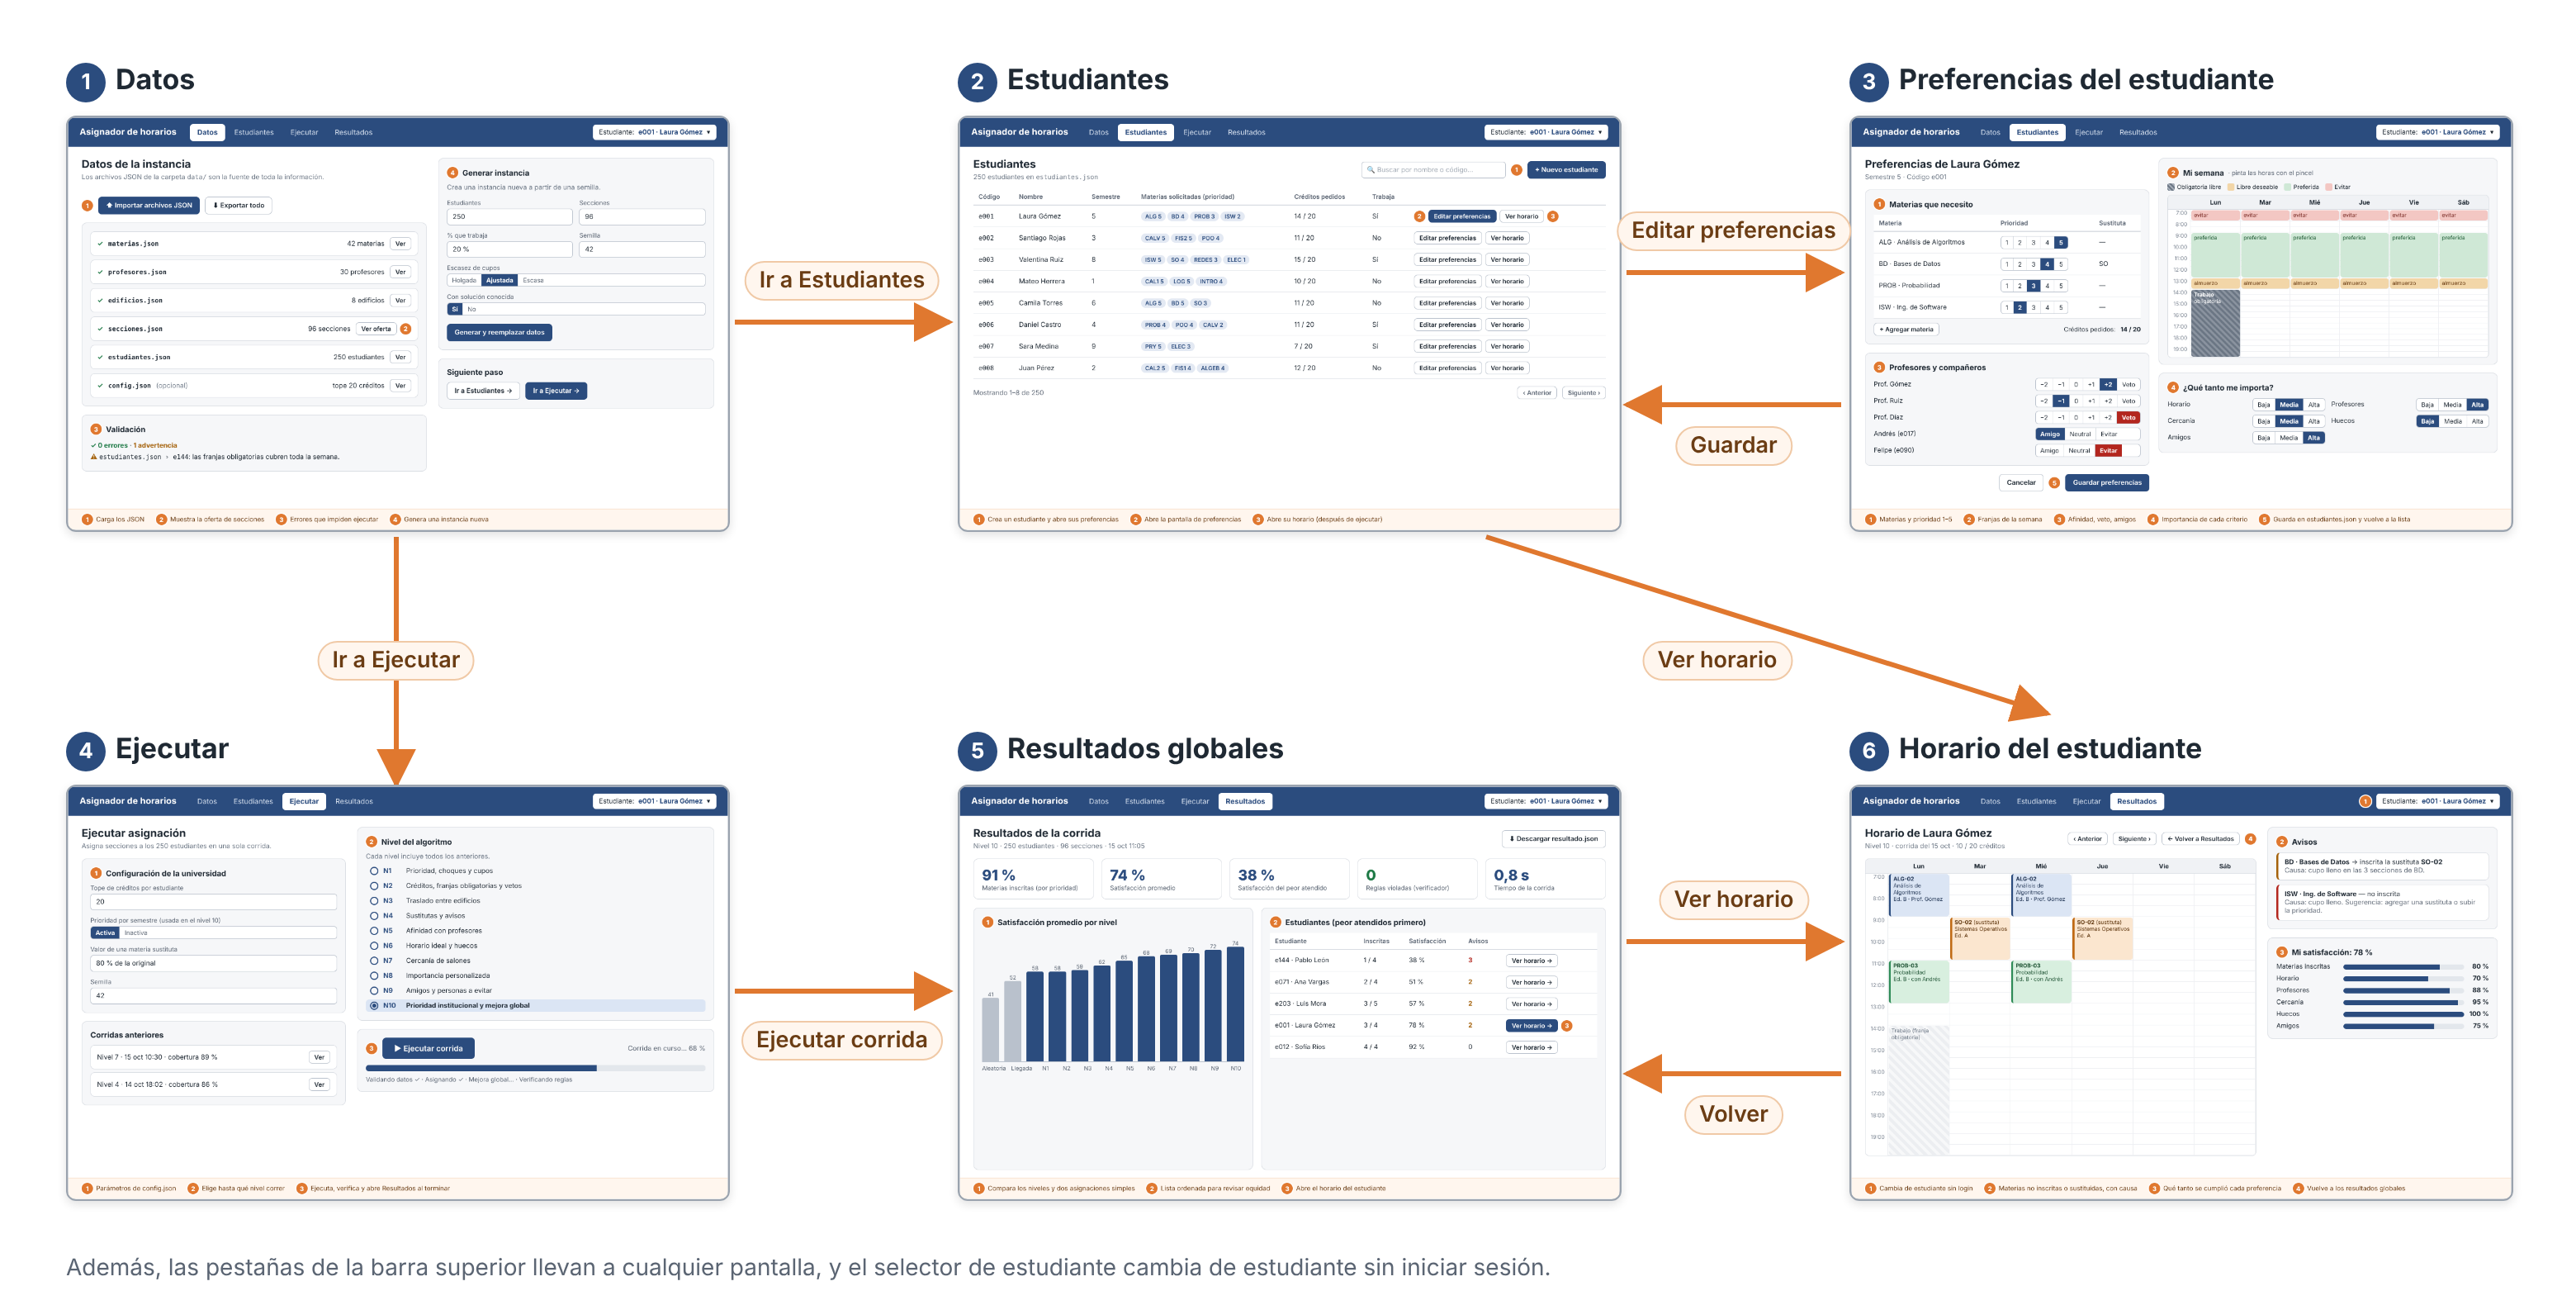
\includegraphics[width=\textwidth]{figuras/mockup_flujo.png}
\caption{Flujo general de la aplicación: seis pantallas y las acciones que llevan de una a otra.}\label{fig:ui-flujo}
\end{figure}

\begin{figure}[htbp]
\centering
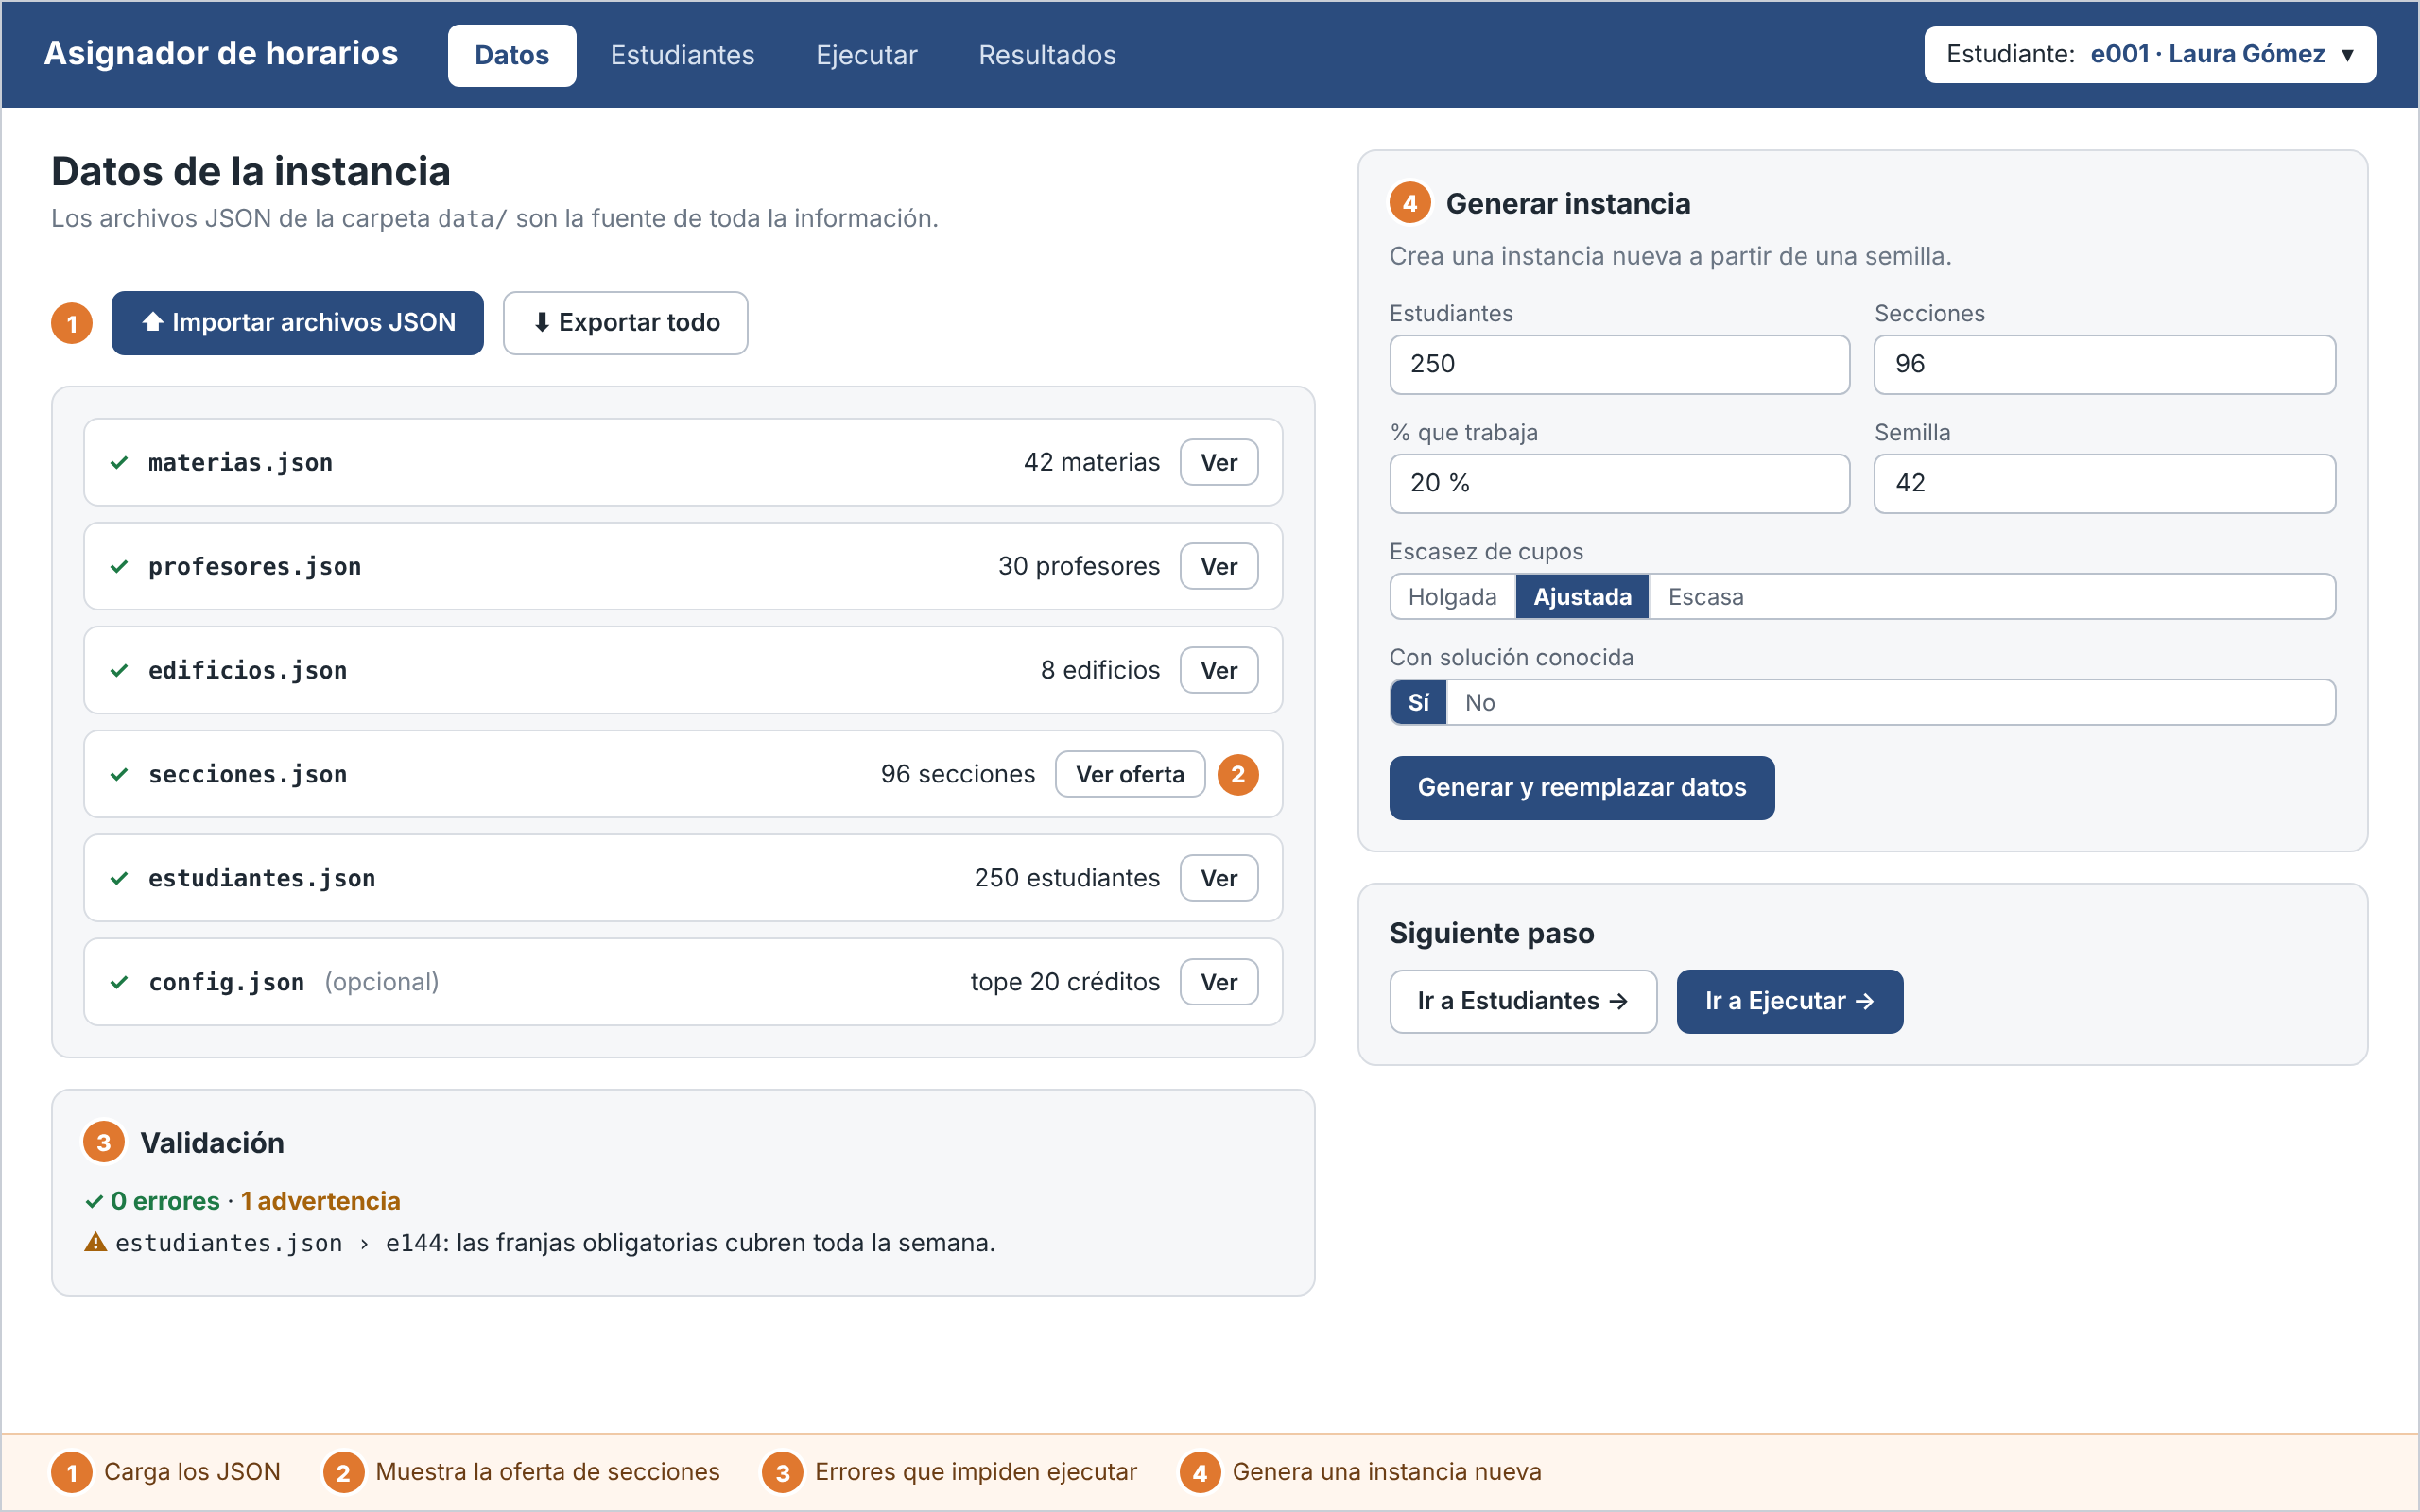
\includegraphics[width=\textwidth]{figuras/mockup1_datos.png}
\caption{Carga de archivos, generación de datos de prueba y revisión de errores.}\label{fig:ui-datos}
\end{figure}

\begin{figure}[htbp]
\centering
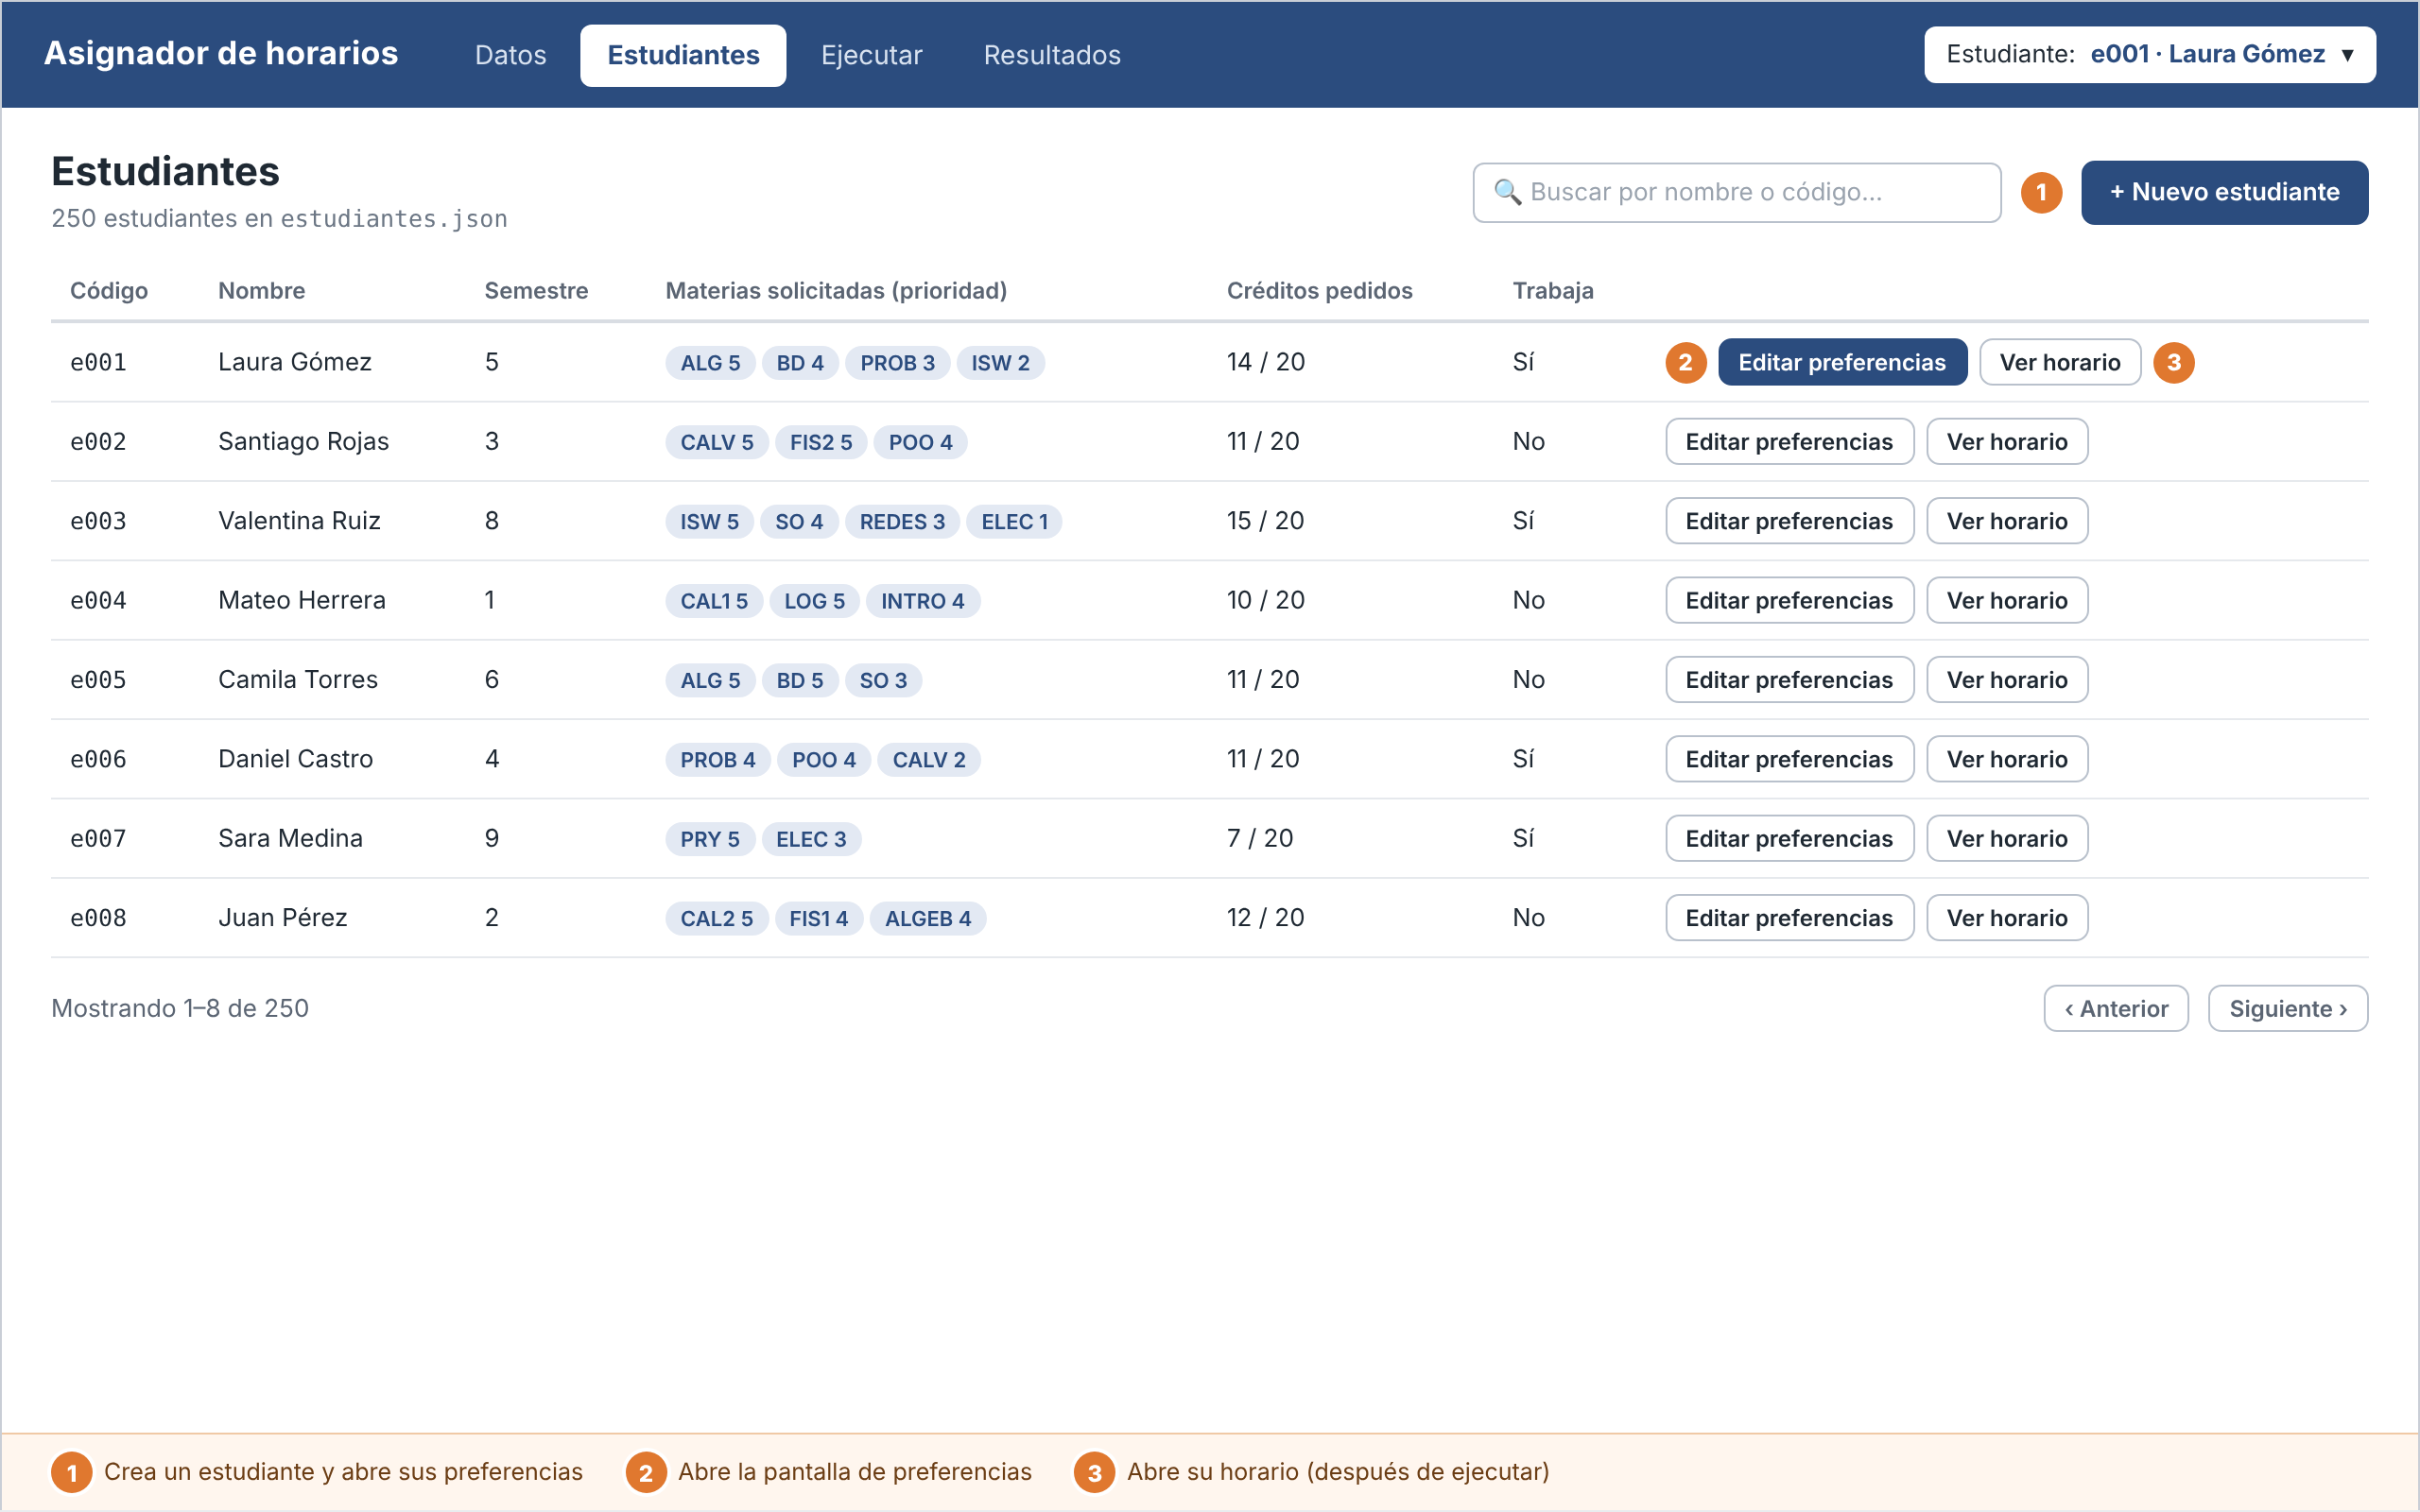
\includegraphics[width=\textwidth]{figuras/mockup2_estudiantes.png}
\caption{Lista de estudiantes con sus materias, prioridades y créditos pedidos.}\label{fig:ui-estudiantes}
\end{figure}

\begin{figure}[htbp]
\centering
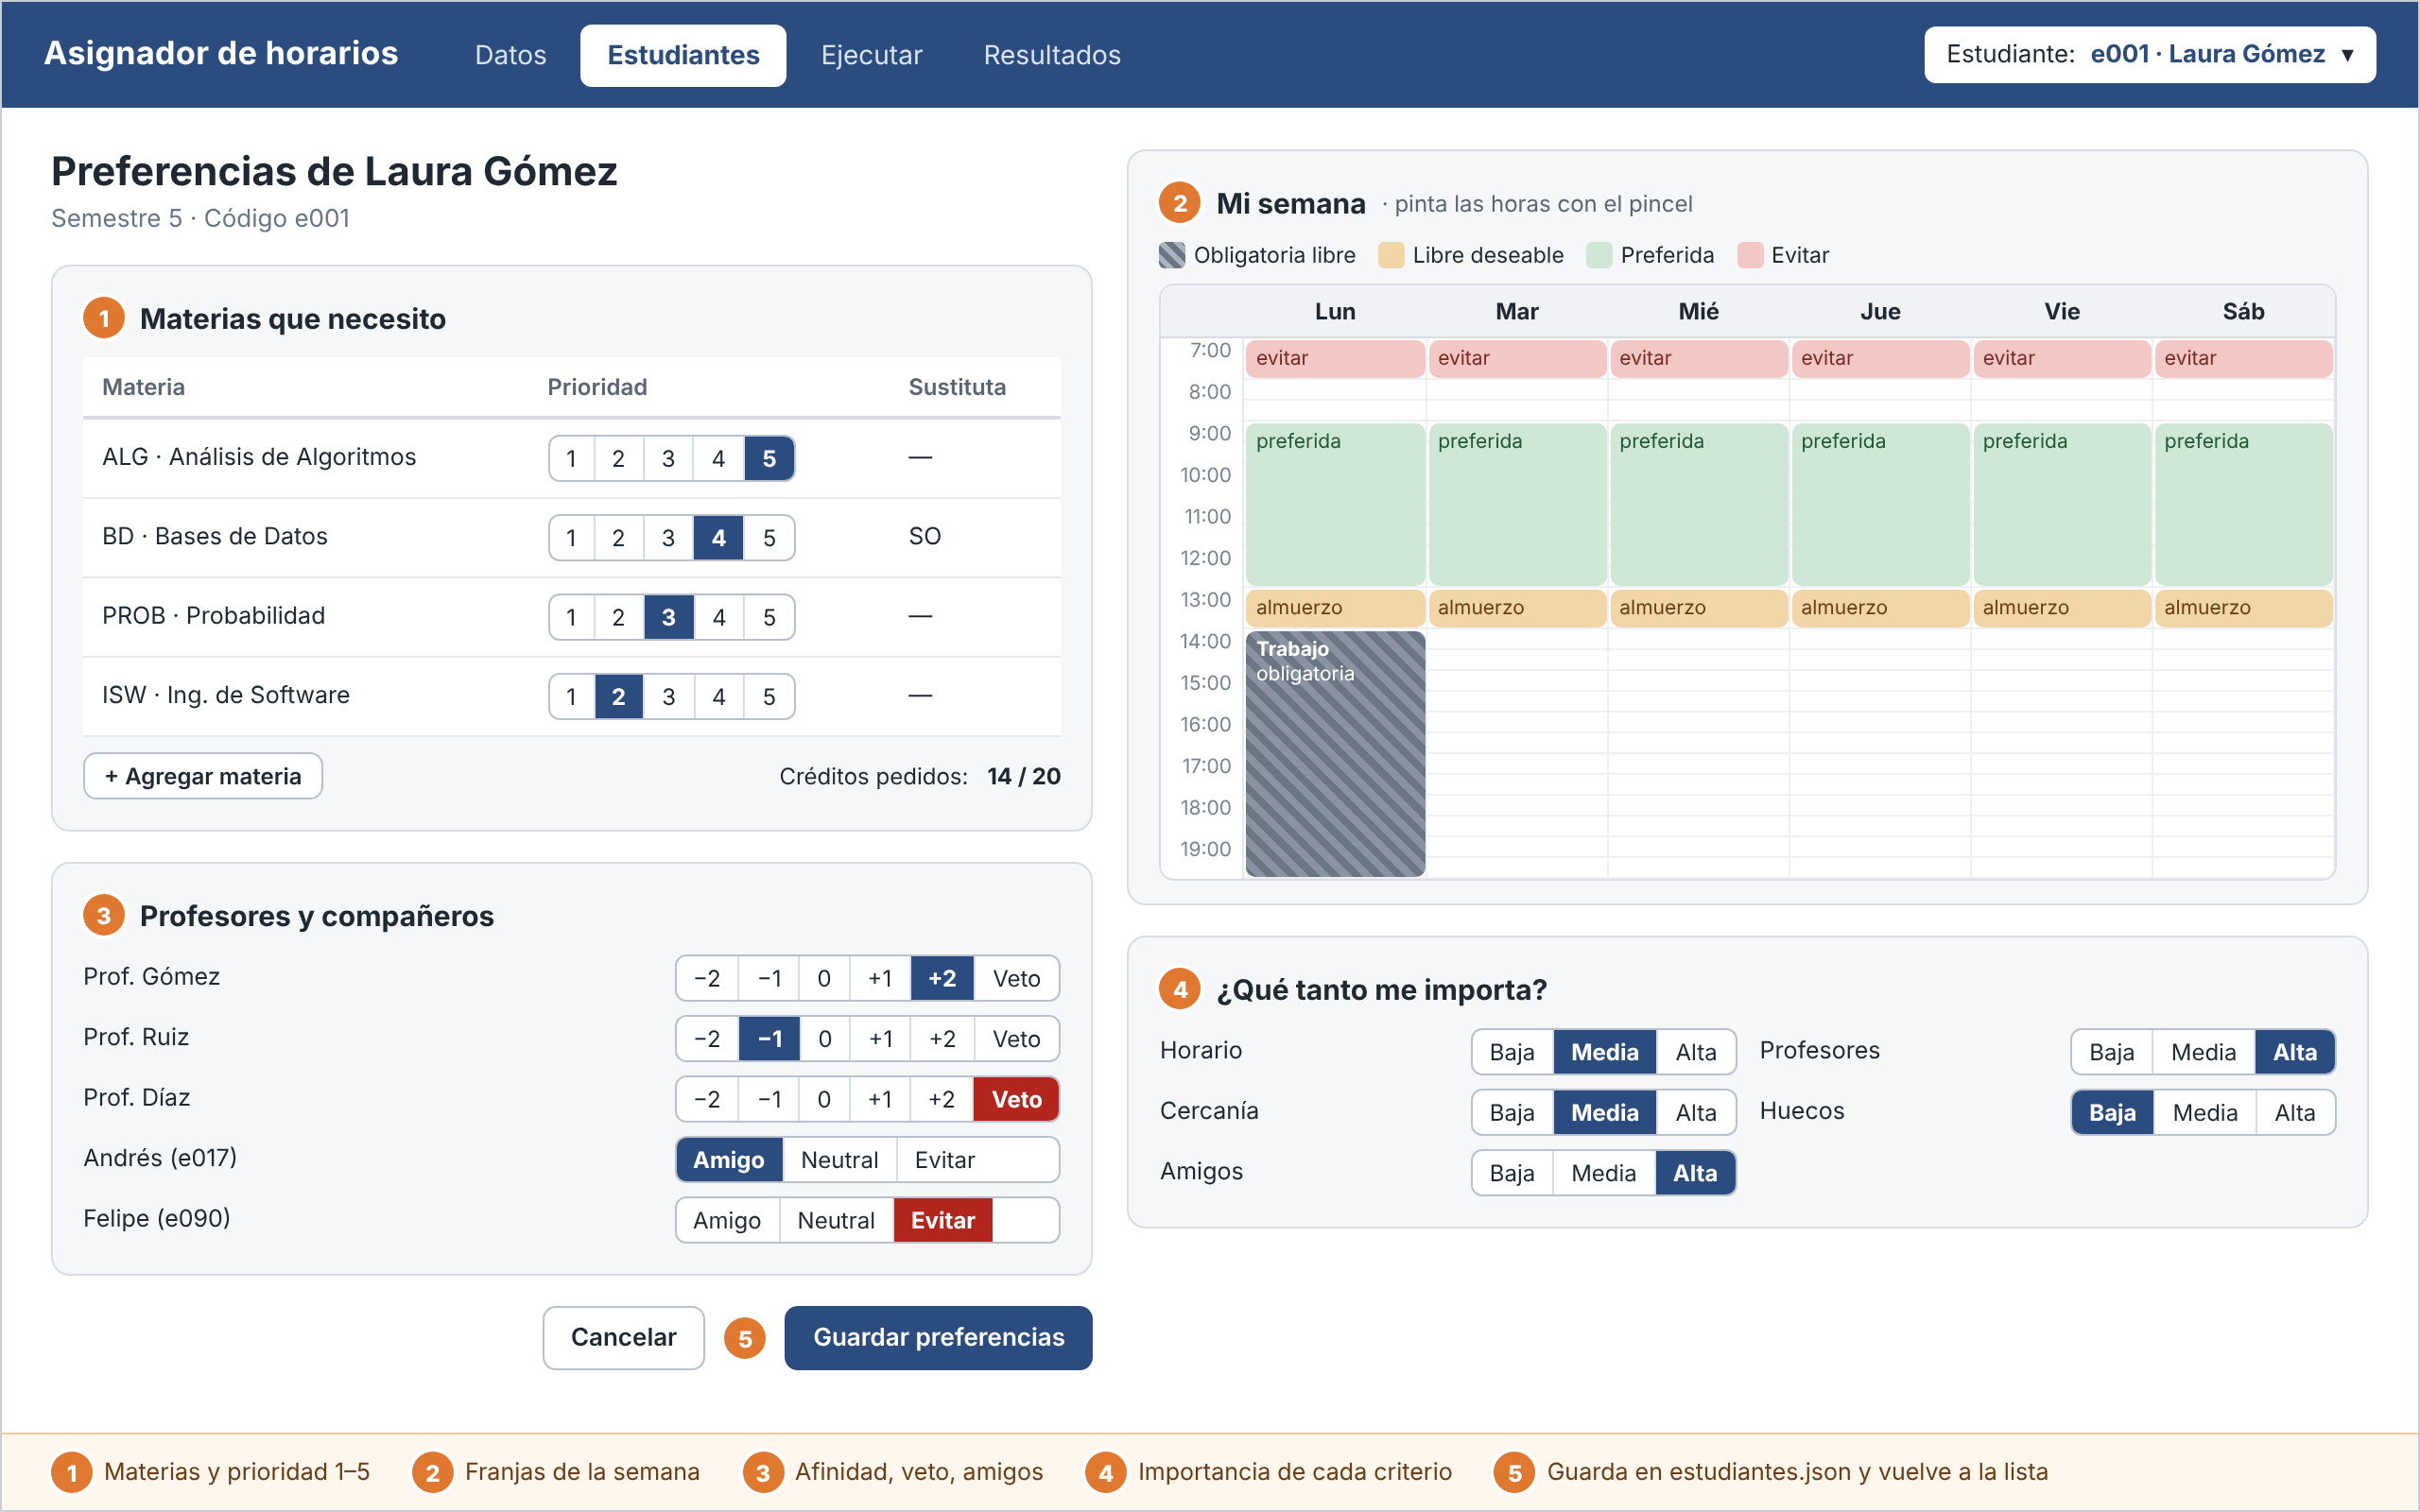
\includegraphics[width=\textwidth]{figuras/mockup3_preferencias.png}
\caption{Selección de materias y prioridades, franjas horarias, profesores y compañeros.}\label{fig:ui-preferencias}
\end{figure}

\begin{figure}[htbp]
\centering
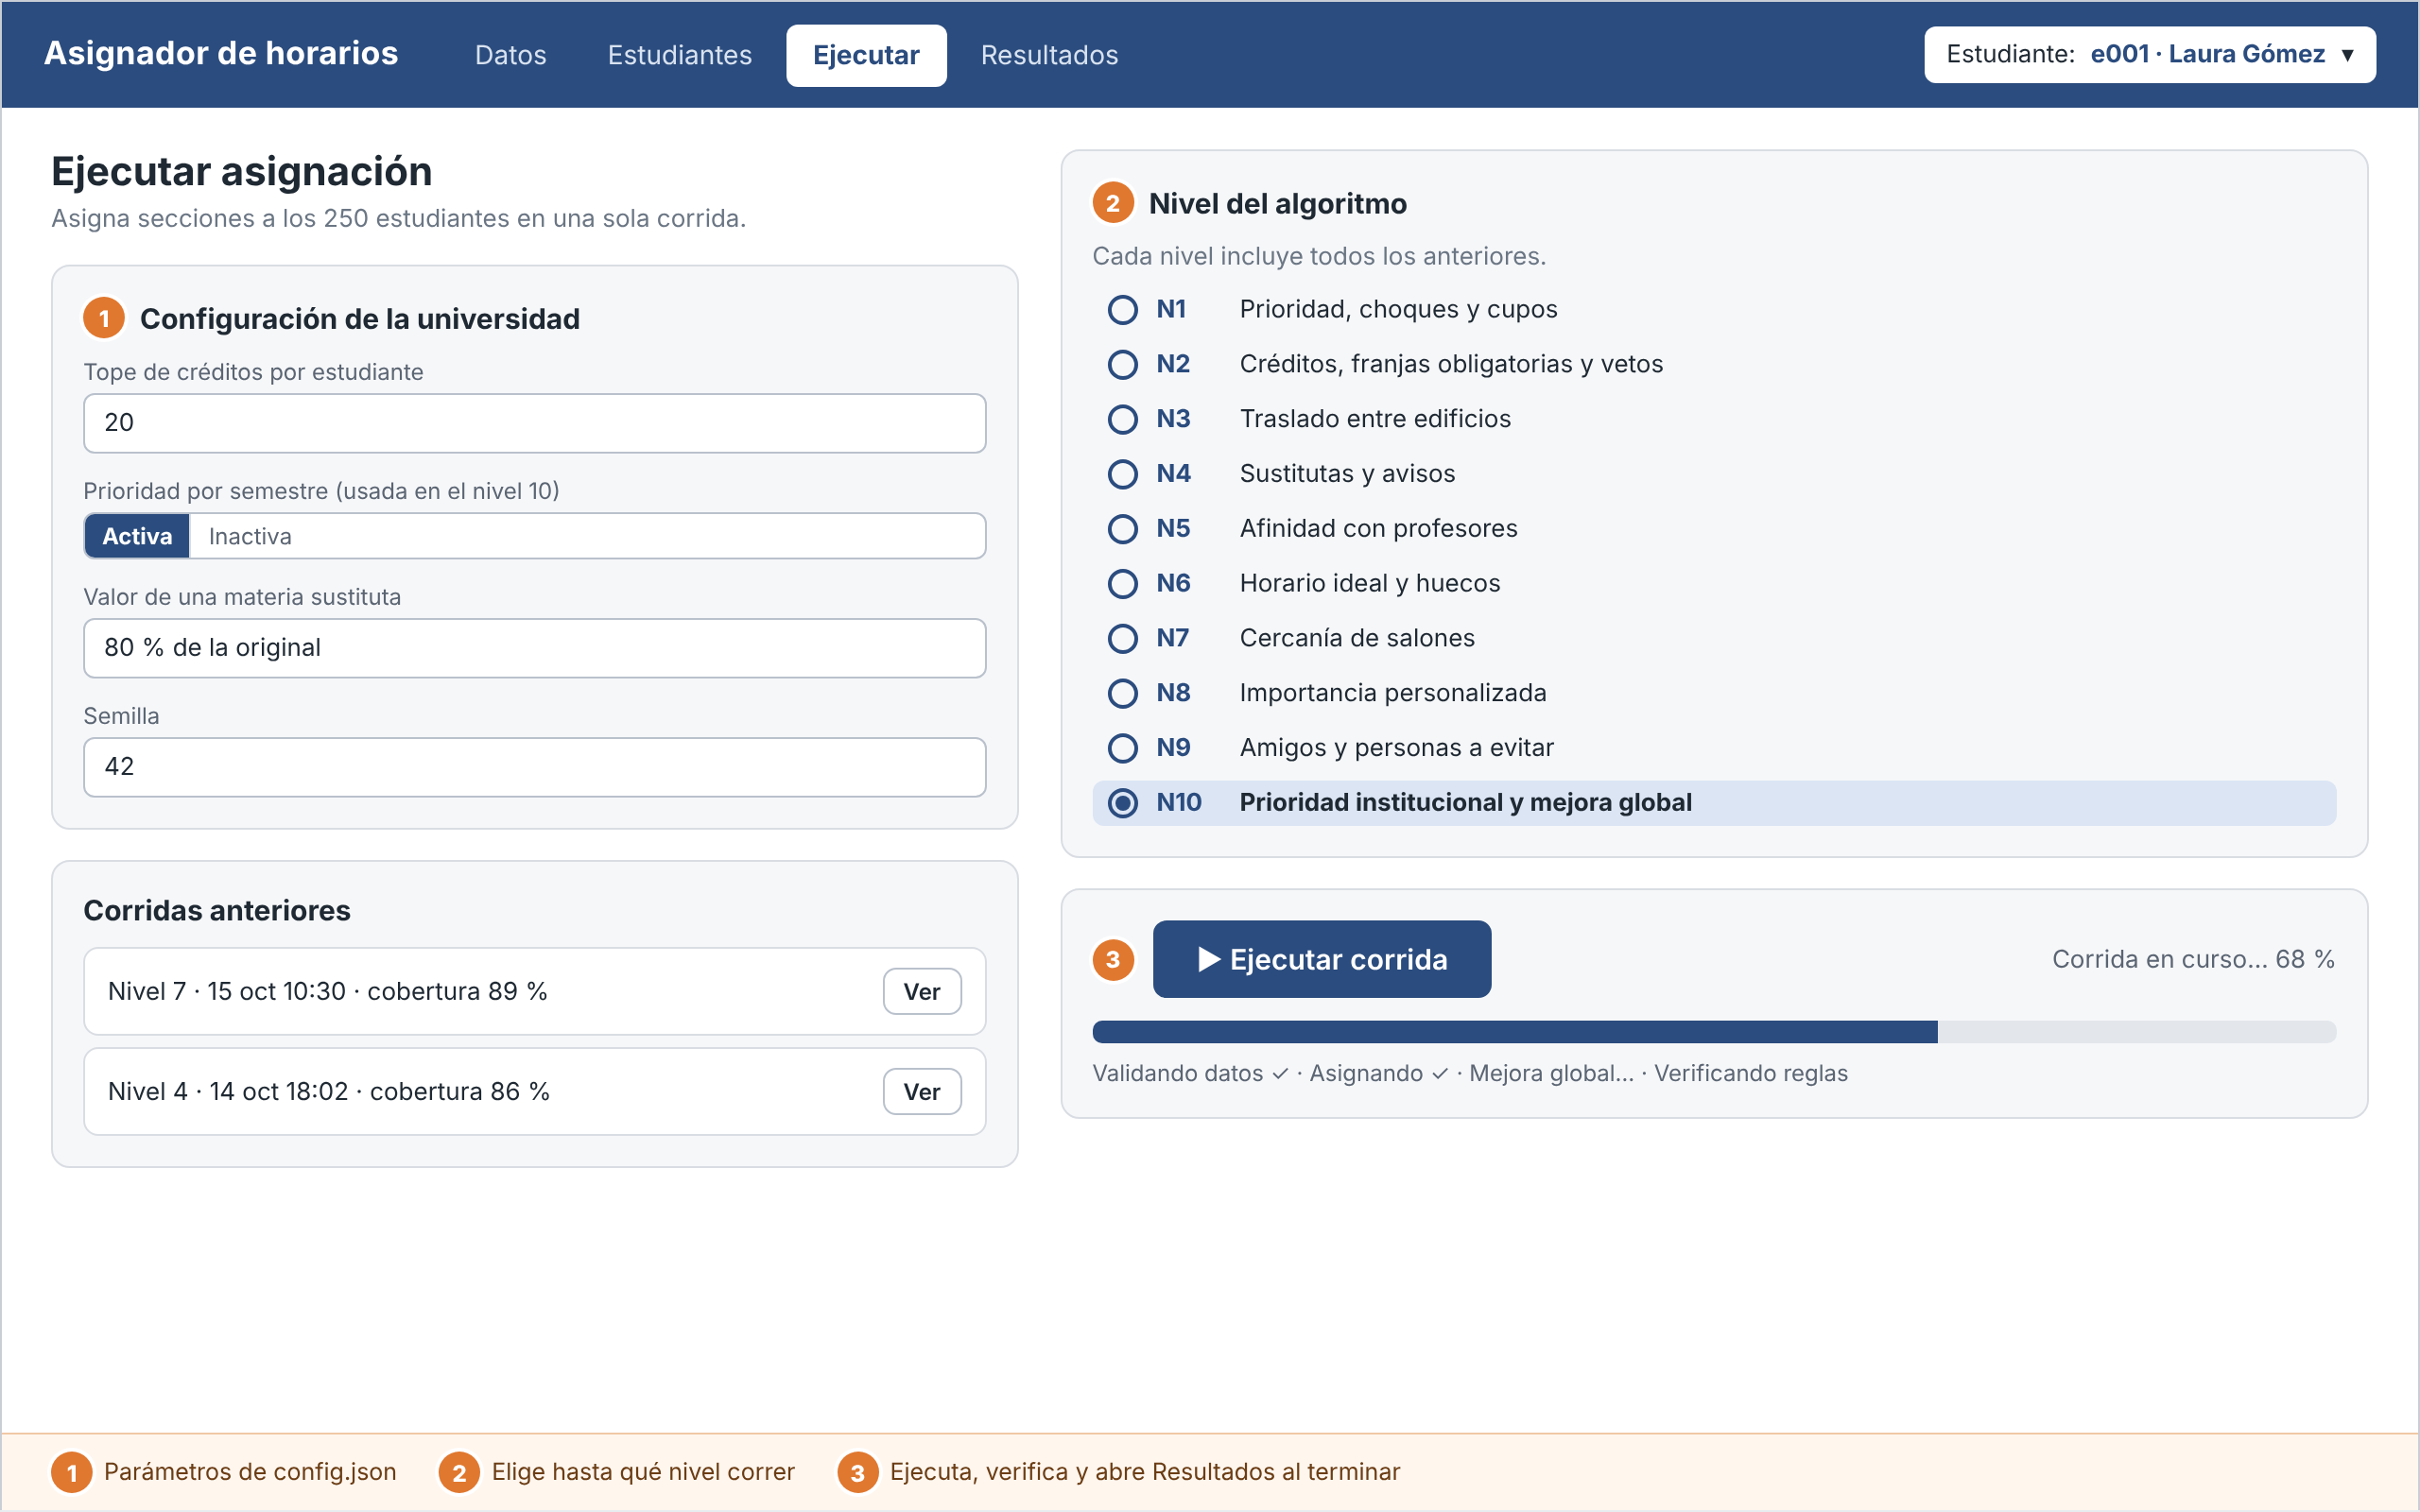
\includegraphics[width=\textwidth]{figuras/mockup4_ejecutar.png}
\caption{Configuración de la universidad, elección del nivel del algoritmo y ejecución de la corrida.}\label{fig:ui-ejecutar}
\end{figure}

\begin{figure}[htbp]
\centering
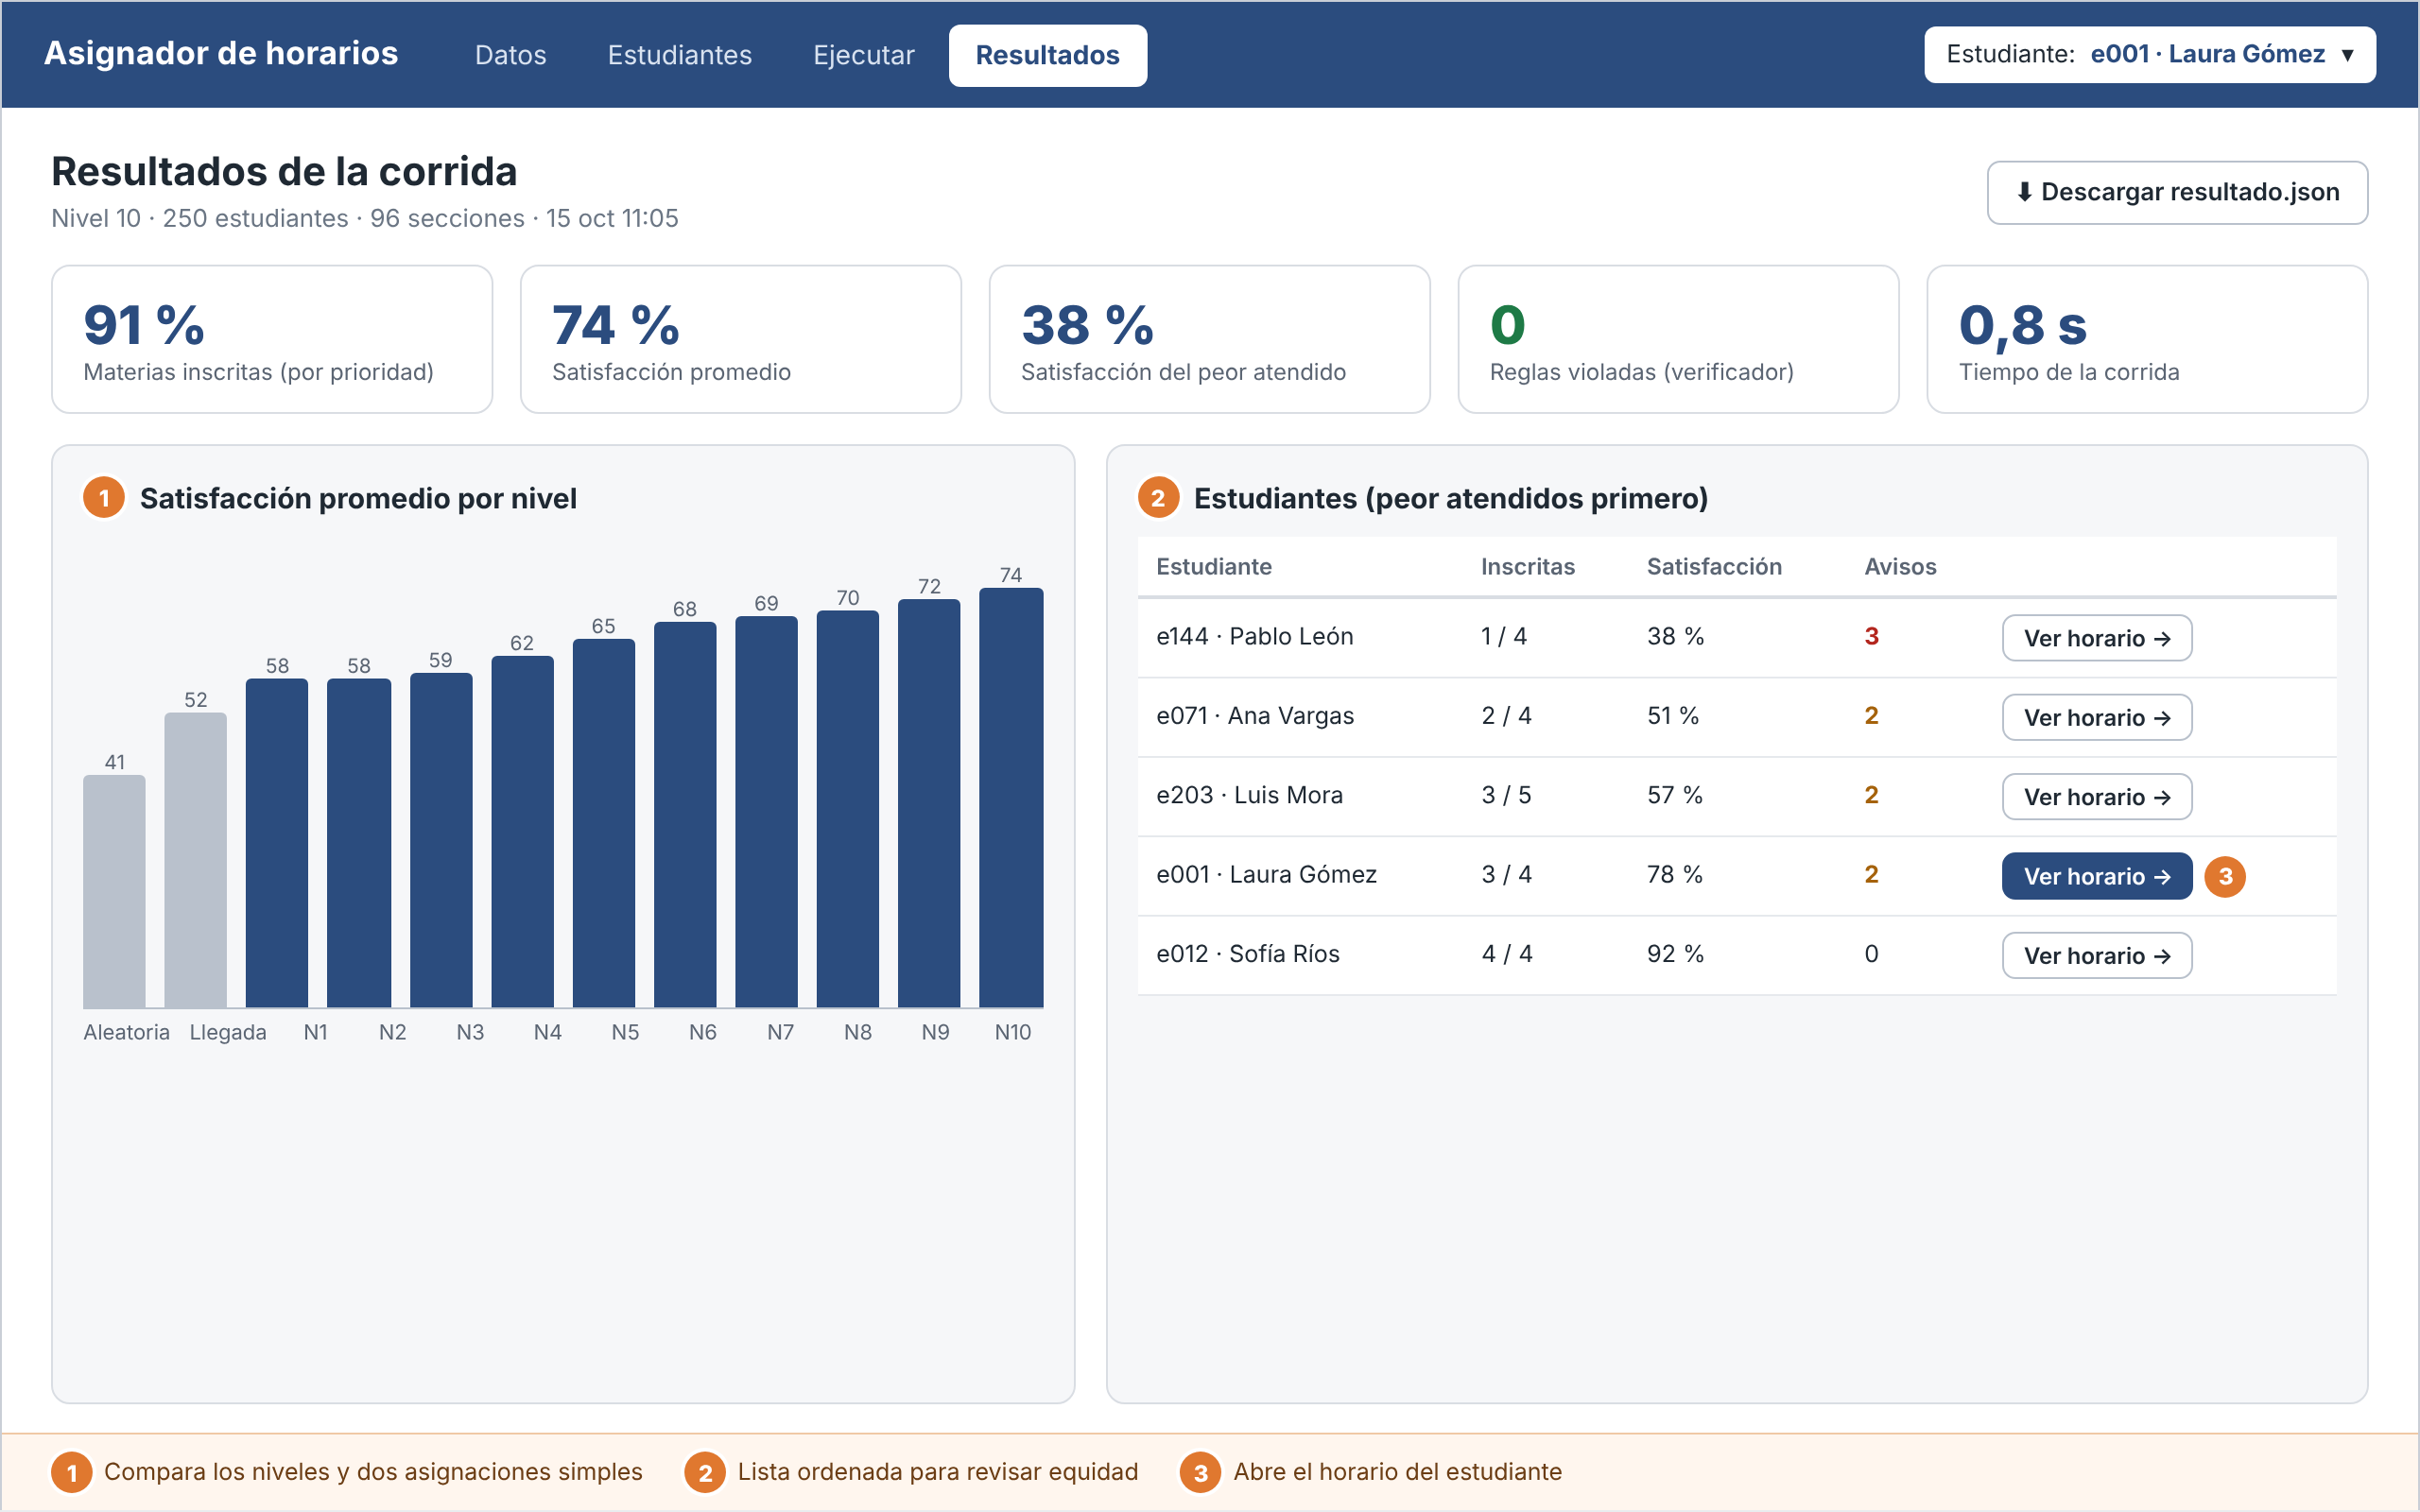
\includegraphics[width=\textwidth]{figuras/mockup5_resultados.png}
\caption{Resultados globales: indicadores de la corrida, comparación entre niveles y estudiantes peor atendidos.}\label{fig:ui-resultados}
\end{figure}

\begin{figure}[htbp]
\centering
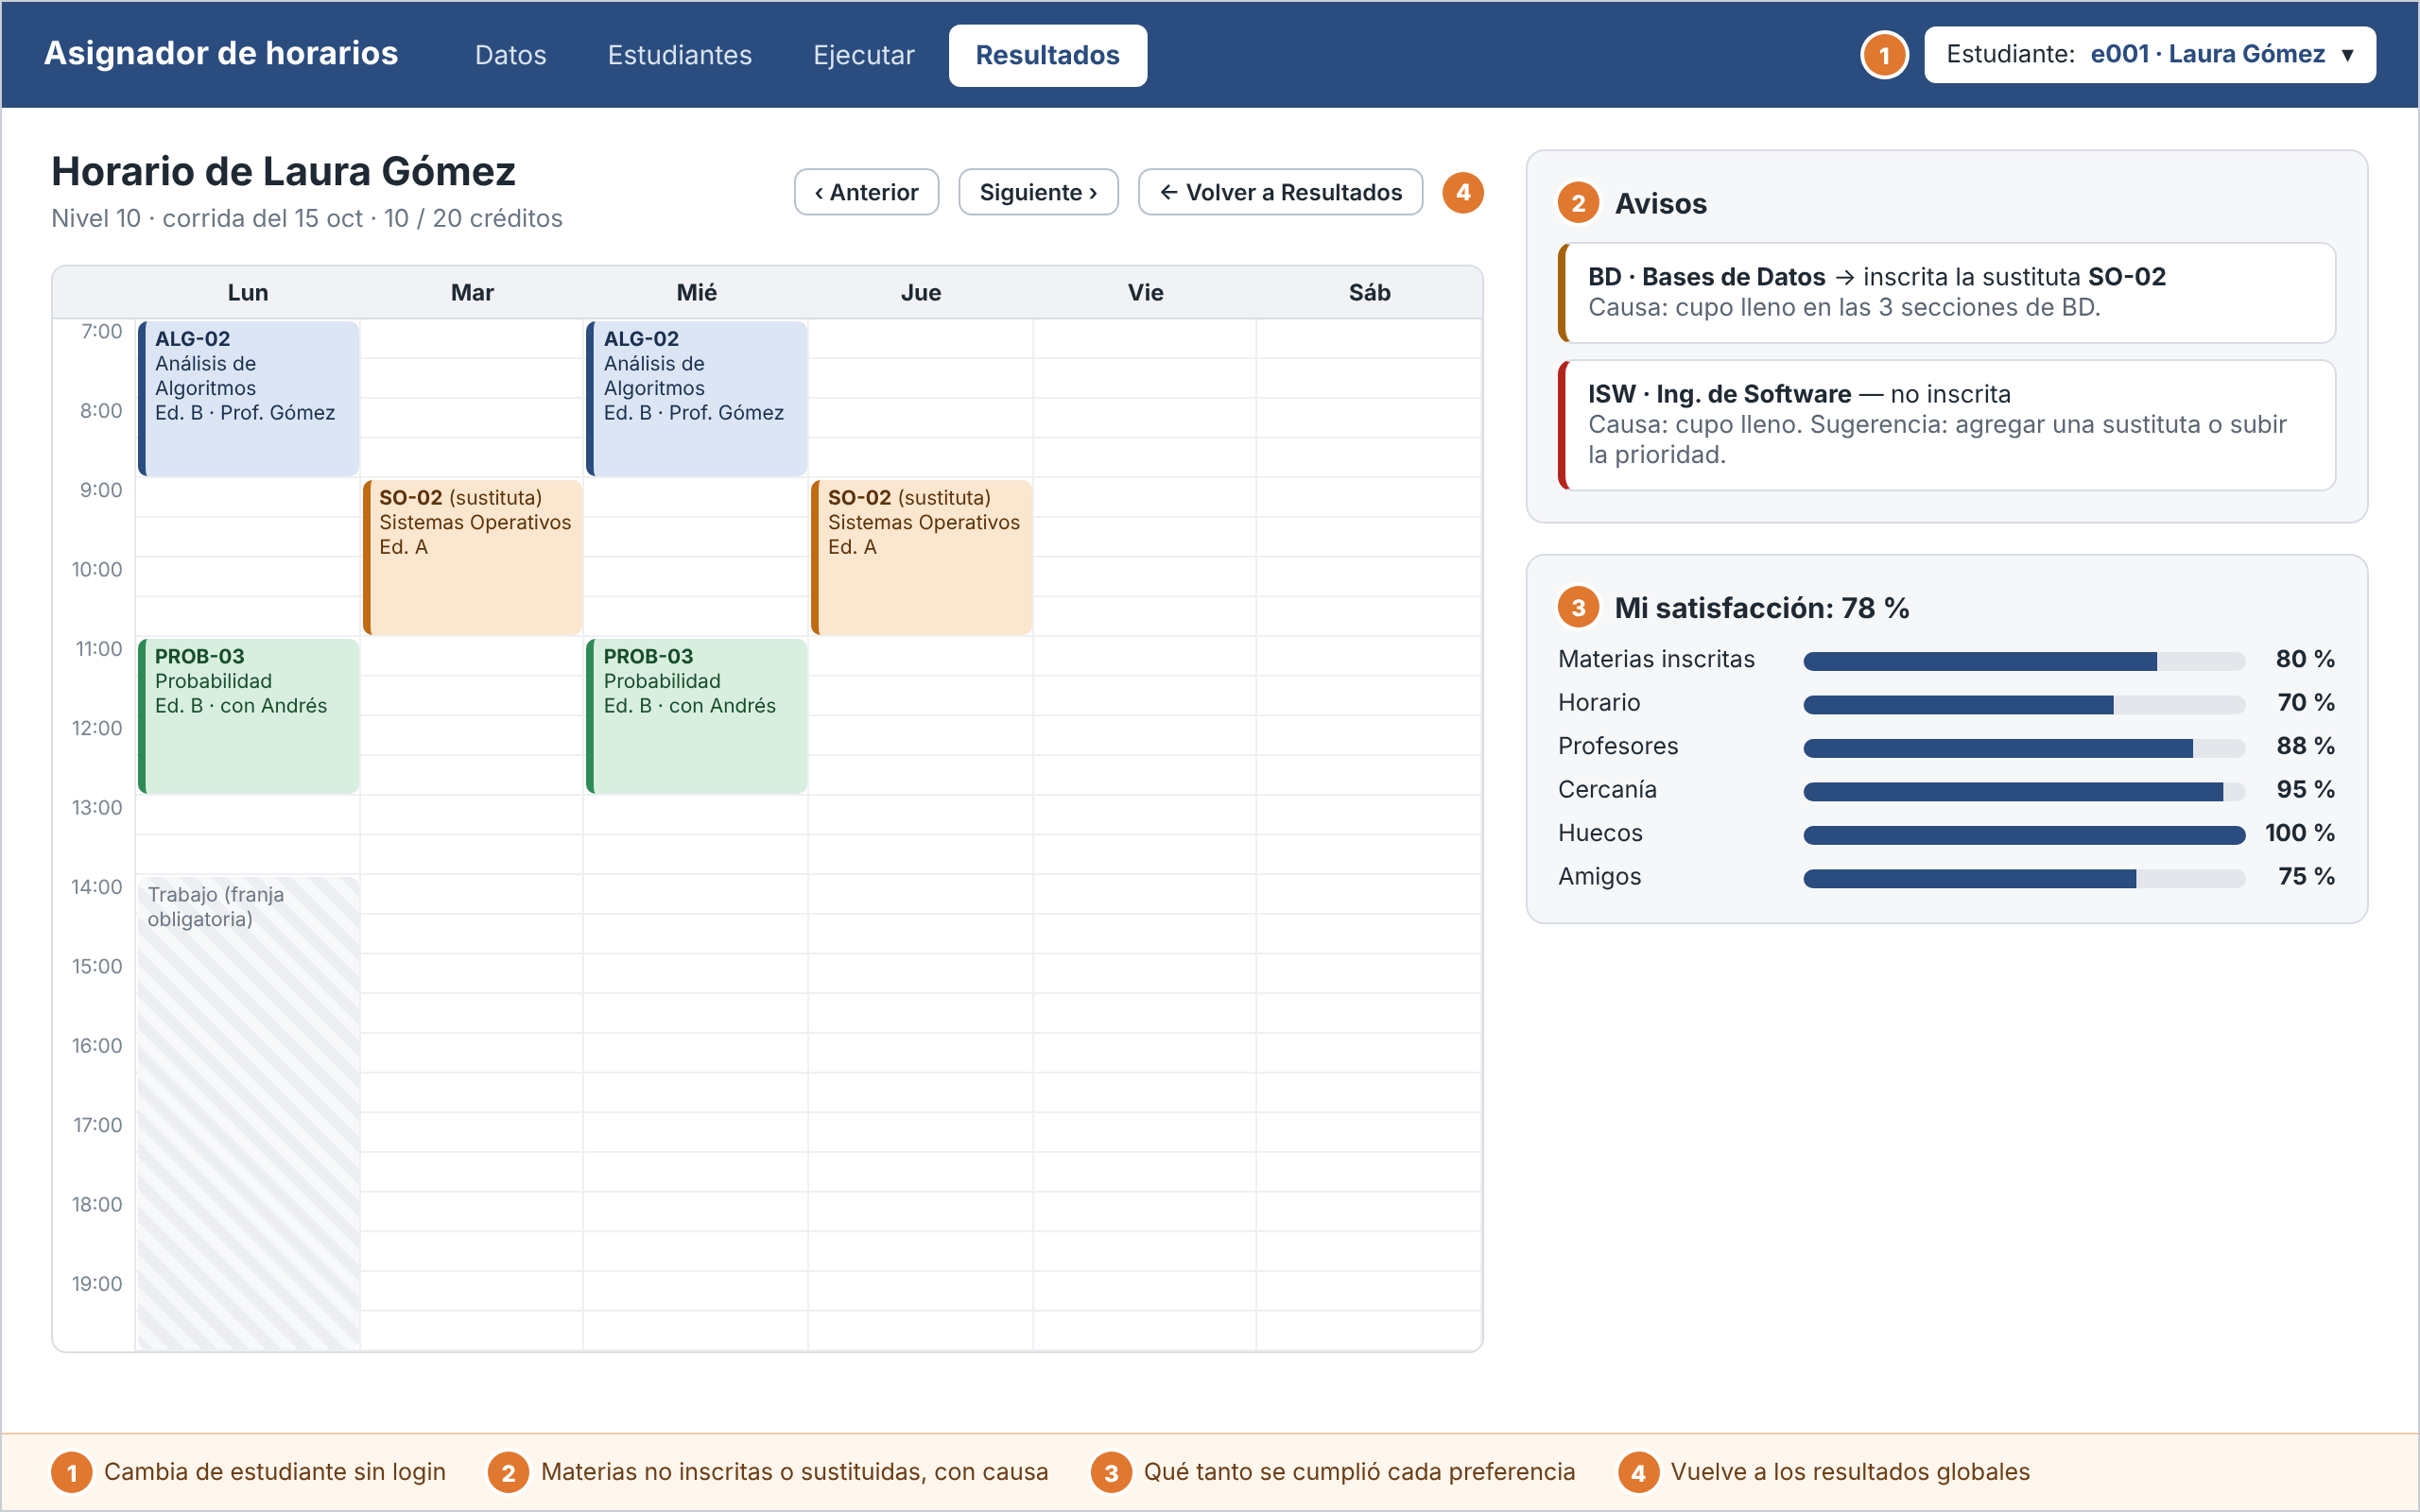
\includegraphics[width=\textwidth]{figuras/mockup6_horario.png}
\caption{Ejemplo de consulta del horario, sustituciones y avisos. Los valores mostrados son ilustrativos.}\label{fig:ui-horario}
\end{figure}

% TODO (Andrés): describir la aplicación implementada (y, si se puede, reemplazar los mockups por capturas reales).
% Indicar si se separaron las etiquetas de materias atendidas y satisfacción, si la carga de datos incluye traslados.json
% y el estado de la pantalla de Preferencias. Borrar la nota en rojo al completar.
\textcolor{red}{[Pendiente: descripción de la aplicación implementada y capturas de pantalla.]}
